% !TeX options = -shell-escape

\documentclass[10pt]{beamer}

\usetheme[progressbar=frametitle, block=fill]{metropolis}
\usepackage{xcolor}
\usepackage{multirow}
\usepackage{pgfpages}
\usepackage{pifont}
\usepackage{textpos}
\newcommand{\cmark}{\ding{51}}
\newcommand{\xmark}{\ding{55}}
\setbeamertemplate{note page}{\insertnote}
%\setbeameroption{show notes on second screen=left}
\setbeameroption{hide notes}
\definecolor{amethyst}{rgb}{0.5, 0.4, 1.0}
\definecolor{amethystgrey}{rgb}{0.85, 0.85, 1.0}
\definecolor{amethystdark}{rgb}{0.4, 0.3, 0.9}
\definecolor{orangedark}{rgb}{0.0, 0.9, 0}
%\definecolor{titlebg}{HTML}{4e8074}
%\definecolor{titlebg}{HTML}{3e7985}
\definecolor{titlebg}{HTML}{fbf8ff}
\definecolor{font}{HTML}{23373b}

%\setbeamercolor{title}{fg=amethyst, bg=amethyst}
\setbeamercolor{frametitle}{fg= font, bg=titlebg}
%\setbeamercolor{section title}{black}
%\setbeamercolor{structure}{fg=amethyst, bg=amethyst}
\setbeamercolor{progress bar}{ fg = amethyst, bg= amethystgrey }
%\setbeamercolor{itemize item}{fg=amethyst,bg=white}
\setbeamercolor{alerted text}{fg=amethystdark}
%\setbeamercolor{title separator}{ ... }
%\setbeamercolor{progress bar in head/foot}{ ... }
%\setbeamercolor{progress bar in section page}{ ... }

\addtobeamertemplate{frametitle}{}{%
\begin{textblock*}{100mm}(1\textwidth, -1cm)

\includegraphics[height=0.97cm]{TT_Logo_bckg.png}
\end{textblock*}}


\usepackage[utf8]{inputenc}
\usepackage[english]{babel}

\usepackage{booktabs}
\usepackage[scale=2]{ccicons}

\usepackage{minted}
\setminted[c++]{linenos = true}

\usepackage{pgfplots}

\usepackage{xspace}

\title{Futuristic Error Handling}
\subtitle{Error handling in C++ today and tomorrow}
%\logo{
\includegraphics[width=0.05\linewidth]{logo.png}}
% \date{\today}
\date{}
\author{Dawid Pilarski}
\institute{dawid.pilarski@panicsofware.com}

\begin{document}

\maketitle

%\begin{frame}{Table of contents}
%  \setbeamertemplate{section in toc}[sections numbered]
%  \tableofcontents[hideallsubsections]
%\end{frame}

\begin{frame}{Why am I here?}
	Why should we bother with error handling?
\end{frame}

\begin{frame}{Recommendable error handling mechanism}
	\note{Q: ask which mechanism would be chosen}
	Which error mechanism would you choose?
	
	There exist two common strategies for error handling:
	\begin{itemize}
		\item error codes
		\item exceptions
	\end{itemize}
\end{frame}

\begin{frame}{Who am I?}
			\centering \alert{Dawid Pilarski}
			\vskip 1em
	\begin{columns}[onlytextwidth]
		\begin{column}{0.7\textwidth}
			\begin{itemize}
				\item Senior Software Developer in TomTom
				\item Member of the ISO/JTC1/SC22/WG21
				\item Member of the PKN KT {\tiny(programming languages)}
				\item C++ blog writer
			\end{itemize}
		\end{column}
		\begin{column}{0.29\textwidth}
				
\includegraphics[width=\linewidth]{Dawid_Pilarski.jpg}				
		\end{column}	
	\end{columns}
\end{frame}

\section{Error codes nowadays}

\begin{frame}{What are the error codes?}
	According to the \alert{Wikipedia} :
	\begin{itemize}[<+- | alert@+>]
		\item error code is an enumerated message,
		\item that corresponds to the status of a specific software application.
		\item They are typically used to identify faults, such as those in faulty hardware, software, or incorrect user input
	\end{itemize}
\end{frame}

\begin{frame}{The error codes.}
	\begin{itemize}[<+- | alert@+>]
		\item Old. C-compatible. Comes from assembly time.
		\item Machine friendly.
		\item Super fast.
		\item Used till today.
	\end{itemize}
\end{frame}

\begin{frame}[fragile]{Error code example}
	\begin{onlyenv}<1->
	\begin{minted}{c++}
int sqlite3_open( const char *filename, sqlite3 **ppDb );
	\end{minted}
	\end{onlyenv}
	
	\begin{onlyenv}<2>
	\hrulefill
	
	\begin{minted}[highlightlines={2,4}]{c++}
int open_status = sqlite3_open(/* ... */ );
if(open_status == SQLITE_OK){
  // make use of opened database
} else if( open_status == SQLITE_CANTOPEN_ISDIR ) {
  // handle the error
}
	\end{minted}
	\end{onlyenv}
	
	\begin{onlyenv}<3>
	\hrulefill

	\begin{minted}[highlightlines={3}]{c++}
int open_status = sqlite3_open(/* ... */ );
if(open_status == SQLITE_OK){
  // make use of opened database
} else if( open_status == SQLITE_CANTOPEN_ISDIR ) {
  // handle the error
}
	\end{minted}

	\end{onlyenv}
	\begin{onlyenv}<4>
	\hrulefill

	\begin{minted}[highlightlines={5}]{c++}
int open_status = sqlite3_open(/* ... */ );
if(open_status == SQLITE_OK){
  // make use of opened database
} else if( open_status == SQLITE_CANTOPEN_ISDIR ) {
  // handle the error
}
\end{minted}
	\end{onlyenv}

\end{frame}

\begin{frame}{Handle the error}
	How to handle the error correctly?
	
	\pause
	
	\begin{itemize}[<+- | alert@+>]
		\item \texttt{std::terminate()}
		\item take the error callback
		\item propagate the error to the caller
	\end{itemize}
	
\end{frame}

\section{Error codes - propagation}

\begin{frame}[fragile]{Propagation}

\begin{onlyenv}<1>
\begin{minted}[highlightlines=1]{c++}
void foo_bar(int& errc /*...*/){
  errc = foo();
  // ...
  errc = bar();		
  // ...
}
	\end{minted}
\end{onlyenv}

\begin{onlyenv}<2>
\begin{minted}[highlightlines={2,4}]{c++}
void foo_bar(int& errc /*...*/){
  errc = foo();
  // ...
  errc = bar();		
  // ...
}
\end{minted}
\end{onlyenv}

\begin{onlyenv}<3>
\begin{minted}[highlightlines={3,6}]{c++}
void foo_bar(foo_bar_errc errc&){
  foo_errc ferrc = foo();
  errc = translate_foo(ferrc);
  // ...
  bar_errc berrc = bar();
  errc = translate_foo(berrc);
}
	\end{minted}
\end{onlyenv}

\begin{onlyenv}<4>
\begin{minted}[highlightlines={4-6}]{c++}
void foo_bar(foo_bar_errc errc&){
  foo_errc ferrc = foo();
  errc = translate_foo(ferrc);
  if(errc != foo_errc::SUCCESS){
  	return;
  }
  // ...
}
	\end{minted}
\end{onlyenv}
\end{frame}

\begin{frame}{C-style error codes summary}
	So we can see {\color{red}serious disadvantages} (except for {\color{blue}obvious advantages}):
	
	\begin{itemize}[<+- | alert@+>]
		\item success path same as error path
		\item cluttering code with translations
		\item boring manual error propagation
	\end{itemize}
\end{frame}
	

\section{Error codes - modern approach}
\begin{frame}{Standard library support - what do we need?}
	\begin{itemize}
		\item A way to define new error codes
		\item A way to distinguish domain of the error codes
	\end{itemize}
\end{frame}

\begin{frame}{Standard library support - what we get?}
	We get three new major types:
	\begin{itemize}[<+- | alert@+>]
		\item std::error\_code
		\item std::error\_category
		\item std::error\_condition
	\end{itemize}
\end{frame}

\begin{frame}[fragile]{std::error\_code in action}
	\begin{onlyenv}<1>
	\begin{minted}[highlightlines={1-2}]{c++}
std::error_code errcode;
is_regular_file("non_existent_directory", errcode);

std::cout << errcode << std::endl;
std::cout << errcode.value() << std::endl;
std::cout << errcode.message() << std::endl;
std::cout << errcode.category().name() << std::endl;
	\end{minted}
	\end{onlyenv}

	\begin{onlyenv}<2>
	\begin{minted}[highlightlines={4}]{c++}
std::error_code errcode;
is_regular_file("non_existent_directory", errcode);

std::cout << errcode << std::endl;
std::cout << errcode.value() << std::endl;
std::cout << errcode.message() << std::endl;
std::cout << errcode.category().name() << std::endl;
	\end{minted}
	\end{onlyenv}

	\begin{onlyenv}<3>
	\begin{minted}[highlightlines={5}]{c++}
std::error_code errcode;
is_regular_file("non_existent_directory", errcode);

std::cout << errcode << std::endl;
std::cout << errcode.value() << std::endl;
std::cout << errcode.message() << std::endl;
std::cout << errcode.category().name() << std::endl;
	\end{minted}
	\end{onlyenv}

	\begin{onlyenv}<4>
	\begin{minted}[highlightlines={6}]{c++}
std::error_code errcode;
is_regular_file("non_existent_directory", errcode);

std::cout << errcode << std::endl;
std::cout << errcode.value() << std::endl;
std::cout << errcode.message() << std::endl;
std::cout << errcode.category().name() << std::endl;
	\end{minted}
	\end{onlyenv}

	\begin{onlyenv}<5>
	\begin{minted}[highlightlines={7}]{c++}
std::error_code errcode;
is_regular_file("non_existent_directory", errcode);

std::cout << errcode << std::endl;
std::cout << errcode.value() << std::endl;
std::cout << errcode.message() << std::endl;
std::cout << errcode.category().name() << std::endl;
	\end{minted}
	\end{onlyenv}
	
	\hrulefill
	
	\begin{onlyenv}<1>
	\begin{block}{output}
	\texttt{\\
		\$ generic:2 \\
		\$ 2 \\
		\$ No such file or directory \\
		\$ generic}	
	\end{block}
	\end{onlyenv}

	\begin{onlyenv}<2>
	\begin{block}{output}
	\texttt{\\
		\$ \alert{generic:2} \\
		\$ 2 \\
		\$ No such file or directory \\
		\$ generic}	
	\end{block}
	\end{onlyenv}
	
	\begin{onlyenv}<3>
	\begin{block}{output}
	\texttt{\\
		\$ generic:2 \\
		\$ \alert{2} \\
		\$ No such file or directory \\
		\$ generic}	
	\end{block}
	\end{onlyenv}

	\begin{onlyenv}<4>
	\begin{block}{output}
	\texttt{\\
		\$ generic:2 \\
		\$ 2 \\
		\$ \alert{No such file or directory} \\
		\$ generic}	
	\end{block}
	\end{onlyenv}

	\begin{onlyenv}<5>
	\begin{block}{output}
	\texttt{\\
		\$ generic:2 \\
		\$ 2 \\
		\$ No such file or directory \\
		\$ \alert{generic}}
	\end{block}
	\end{onlyenv}

\end{frame}

\begin{frame}[fragile]{Acting upon error}
	\begin{onlyenv}<1>
	\begin{minted}[highlightlines={1-2}]{c++}
std::error_code errcode;
is_regular_file("non_existent_file", errcode);
  
if(errcode == errc::no_such_file_or_directory){
  // creating a file
}
	\end{minted}
	\end{onlyenv}

	\begin{onlyenv}<2>
	\begin{minted}[highlightlines={4-6}]{c++}
std::error_code errcode;
is_regular_file("non_existent_file", errcode);
  
if(errcode == errc::no_such_file_or_directory){
  // creating a file
}
	\end{minted}
	\end{onlyenv}

	\begin{onlyenv}<3>
	\centerline{With enum error codes.}
	\vfill
	\begin{minted}[highlightlines={3}]{c++}
void foo_bar(foo_bar_errc errc&){
  foo_errc ferrc = foo();
  errc = translate_foo(ferrc);
  if(errc != foo_errc::SUCCESS){
    return;
  }
  // ...
}
	\end{minted}
	\end{onlyenv}

	\begin{onlyenv}<4>
	\centerline{With std::error\_code.}
	\vfill
	\begin{minted}[highlightlines={3}]{c++}
void foo_bar(std::error_code errc&){
  errc = foo();
  if(errc){
    return;
  }
  // ...
}
	\end{minted}
	\end{onlyenv}

\end{frame}

\begin{frame}{Let's define our own error code}
	Steps to create own error code:
	\begin{itemize}[<+- | alert@+>]
		\item define custom enum with error codes
		\item inform, that the enum is an error code
		\item create custom error category
		\item create enum to error code factory function
		\item define custom error condition
		\begin{itemize}
			\item define error condition enum
			\item inform the world about new error condition enum
			\item create custom error category for condition enum
			\item make conversion function from new error condition enum to error condition
		\end{itemize}
		\item enjoy!
	\end{itemize}
\end{frame}

\section{Error codes - \\ defining custom error codes}

\begin{frame}[fragile]{Step 1 - define custom enum with error codes}
	\begin{onlyenv}<1>
	\begin{minted}[highlightlines={2}]{c++}
enum class open_file_error {
  SUCCESS, // zero means success
  NO_SUCH_FILE_OR_DIRECTORY,
  FILE_IS_DIRECTORY,
  LACK_OF_RESOURCES,
  FILE_BROKEN,
  NO_PERMISSIONS
};
	\end{minted}
	\end{onlyenv}

	\begin{onlyenv}<2>
	\begin{minted}[highlightlines={3,4}]{c++}
enum class open_file_error {
  SUCCESS, // zero means success
  NO_SUCH_FILE_OR_DIRECTORY,
  FILE_IS_DIRECTORY,
  LACK_OF_RESOURCES,
  FILE_BROKEN,
  NO_PERMISSIONS
};
\end{minted}
	\end{onlyenv}

	\begin{onlyenv}<3>
	\begin{minted}[highlightlines={5,6}]{c++}
enum class open_file_error {
  SUCCESS, // zero means success
  NO_SUCH_FILE_OR_DIRECTORY,
  FILE_IS_DIRECTORY,
  LACK_OF_RESOURCES,
  FILE_BROKEN,
  NO_PERMISSIONS
};
\end{minted}
	\end{onlyenv}

	\begin{onlyenv}<4>
	\begin{minted}[highlightlines={7}]{c++}
enum class open_file_error {
  SUCCESS, // zero means success
  NO_SUCH_FILE_OR_DIRECTORY,
  FILE_IS_DIRECTORY,
  LACK_OF_RESOURCES,
  FILE_BROKEN,
  NO_PERMISSIONS
};
\end{minted}
	\end{onlyenv}

\end{frame}

\begin{frame}[fragile]{Step 2 - inform the world about new error code type}
\begin{minted}{c++}
namespace std{
  template <> struct
  is_error_code_enum<open_file_error> : std::true_type{};
}
\end{minted}
	
\end{frame}

\begin{frame}[fragile]{Step 3 - custom error category}
	
	\begin{minted}{c++}
struct open_file_error_domain : std::error_category {
  const char *name() const noexcept override;		
  std::string message(int errc) const override;
};
	\end{minted}
\end{frame}

\begin{frame}[fragile]{Step 3 - custom error category}
\begin{minted}{c++}
const char* open_file_error_domain::name() const noexcept{
  return "Open File Error";
}
\end{minted}
\end{frame}

\begin{frame}[fragile]{Step 3 - custom error category}
	\begin{onlyenv}<1>
	\begin{minted}[highlightlines={3}]{c++}
std::string open_file_error_domain::message(int errc) const{
  if(errc < 0 or errc > 4) return "UNKNOWN ERROR";
  switch (static_cast<open_file_error>(errc)){
    case open_file_error::SUCCESS:
      return "Success.";
    case open_file_error::NO_SUCH_FILE_OR_DIRECTORY:
      return "File does not exist.";
    // other cases
    case open_file_error::NO_PERMISSIONS:
      return "Missing permissions to open the file."
  }
}
	\end{minted}
	\end{onlyenv}

	\begin{onlyenv}<2>
	\begin{minted}[highlightlines={4,5}]{c++}
std::string open_file_error_domain::message(int errc) const{
  if(errc < 0 or errc > 4) return "UNKNOWN ERROR";
  switch (static_cast<open_file_error>(errc)){
    case open_file_error::SUCCESS:
      return "Success.";
    case open_file_error::NO_SUCH_FILE_OR_DIRECTORY:
      return "File does not exist.";
    // other cases
    case open_file_error::NO_PERMISSIONS:
      return "Missing permissions to open the file."
  }
}
	\end{minted}
	\end{onlyenv}

	\begin{onlyenv}<3>
	\begin{minted}[highlightlines={6,7}]{c++}
std::string open_file_error_domain::message(int errc) const{
  if(errc < 0 or errc > 4) return "UNKNOWN ERROR";
  switch (static_cast<open_file_error>(errc)){
    case open_file_error::SUCCESS:
      return "Success.";
    case open_file_error::NO_SUCH_FILE_OR_DIRECTORY:
      return "File does not exist.";
    // other cases
    case open_file_error::NO_PERMISSIONS:
      return "Missing permissions to open the file."
  }
}
\end{minted}
	\end{onlyenv}

	\begin{onlyenv}<4>
	\begin{minted}[highlightlines={8-10}]{c++}
std::string open_file_error_domain::message(int errc) const{
  if(errc < 0 or errc > 4) return "UNKNOWN ERROR";
  switch (static_cast<open_file_error>(errc)){
    case open_file_error::SUCCESS:
      return "Success.";
    case open_file_error::NO_SUCH_FILE_OR_DIRECTORY:
      return "File does not exist.";
    // other cases
    case open_file_error::NO_PERMISSIONS:
      return "Missing permissions to open the file."
  }
}
\end{minted}
	\end{onlyenv}

	\begin{onlyenv}<5>
	\begin{minted}[highlightlines={2}]{c++}
std::string open_file_error_domain::message(int errc) const{
  if(errc < 0 or errc > 4) return "UNKNOWN ERROR";
  switch (static_cast<open_file_error>(errc)){
    case open_file_error::SUCCESS:
      return "Success.";
    case open_file_error::NO_SUCH_FILE_OR_DIRECTORY:
      return "File does not exist.";
    // other cases
    case open_file_error::NO_PERMISSIONS:
      return "Missing permissions to open the file."
  }
}
\end{minted}
	\end{onlyenv}
\end{frame}

\begin{frame}[fragile]{Step 4 - factory function}
	\begin{onlyenv}<1>
	\begin{minted}[highlightlines={3}]{c++}
namespace std{
  template <typename ErrorCode>
  error_code::error_code(typename std::enable_if<
                                  is_error_code_enum<
                                      ErrorCode>
                                  ::value, ErrorCode>
                         ::type errcode) noexcept 
             : error_code(make_error_code(errcode))
  {}
}
	\end{minted}
	\end{onlyenv}

	\begin{onlyenv}<2>
	\begin{minted}[highlightlines={4-7}]{c++}
namespace std{
  template <typename ErrorCode>
  error_code::error_code(typename std::enable_if<
                                  is_error_code_enum<
                                      ErrorCode>
                                  ::value, ErrorCode>
                         ::type errcode) noexcept 
             : error_code(make_error_code(errcode))
  {}
}
	\end{minted}
	\end{onlyenv}
	
	\begin{onlyenv}<3>
	\begin{minted}[highlightlines={8}]{c++}
namespace std{
  template <typename ErrorCode>
  error_code::error_code(typename std::enable_if<
                                  is_error_code_enum<
                                      ErrorCode>
                                  ::value, ErrorCode>
                         ::type errcode) noexcept 
             : error_code(make_error_code(errcode))
  {}
}
	\end{minted}
	\end{onlyenv}

\end{frame}

\begin{frame}[fragile]{Step 4 - factory function}
	\begin{minted}{c++}
std::error_code make_error_code(open_file_error errc){
  return {static_cast<int>(errc), open_file_error_domain};
}
	\end{minted}
\end{frame}

\begin{frame}[fragile]{Step 5 - custom error condition}
	\begin{minted}{c++}
enum class library_error_condition{
  SUCCESS,
  WRONG_ARGUMENT,
  OS_ERROR,
  PERMISSIONS_ERROR
};
	\end{minted}

	\begin{onlyenv}<2>
	\hrule
	\vfill

	\begin{minted}[fontsize=\footnotesize]{c++}
enum class open_file_error {
  SUCCESS, // zero means success
  NO_SUCH_FILE_OR_DIRECTORY,
  FILE_IS_DIRECTORY,
  LACK_OF_RESOURCES,
  FILE_BROKEN,
  NO_PERMISSIONS
};
	\end{minted}

	\end{onlyenv}

\end{frame}

\begin{frame}[fragile]{Step 5 - custom error condition}
	\begin{minted}{c++}

namespace std{
  template <> struct
  is_error_condition_enum<library_error_condition>
                             : std::true_type{};
}
	\end{minted}
\end{frame}

\begin{frame}[fragile]{Step 5 - custom error condition}
	\begin{minted}{c++}
struct library_error_domain : std::error_category{
  const char *name() const noexcept override;
  std::string message(int errc) const override;
  bool equivalent(const std::error_code &errc, int condition) 
                                      const noexcept override;
};
	\end{minted}
\end{frame}

\begin{frame}[fragile]{Step 5 - custom error condition}
	\begin{onlyenv}<1>
	\begin{minted}[highlightlines={4}]{c++}
bool library_error_domain::equivalent(
          const std::error_code &errc, int condition) 
                                      const noexcept{                     
  switch (static_cast<library_error_condition>(condition)){
    case library_error::SUCCESS:
      if(errc == open_file_error::SUCCESS)
        return true;
    case library_error::WRONG_ARGUMENT:
      if(errc == 
           open_file_error::NO_SUCH_FILE_OR_DIRECTORY or
         errc == 
           open_file_error::FILE_IS_DIRECTORY)
        return true;
    //other cases    
  }
  return false;
}
	\end{minted}
	\end{onlyenv}

	\begin{onlyenv}<2>
	\begin{minted}[highlightlines={5-7}]{c++}
bool library_error_domain::equivalent(
          const std::error_code &errc, int condition) 
                                      const noexcept{                     
  switch (static_cast<library_error_condition>(condition)){
    case library_error::SUCCESS:
      if(errc == open_file_error::SUCCESS)
        return true;
    case library_error::WRONG_ARGUMENT:
      if(errc == 
           open_file_error::NO_SUCH_FILE_OR_DIRECTORY or
         errc == 
           open_file_error::FILE_IS_DIRECTORY)
        return true;
    //other cases    
  }
  return false;
}
	\end{minted}
	\end{onlyenv}

	\begin{onlyenv}<3>
	\begin{minted}[highlightlines={8-13}]{c++}
bool library_error_domain::equivalent(
          const std::error_code &errc, int condition) 
                                      const noexcept{                     
  switch (static_cast<library_error_condition>(condition)){
    case library_error::SUCCESS:
      if(errc == open_file_error::SUCCESS)
        return true;
    case library_error::WRONG_ARGUMENT:
      if(errc == 
           open_file_error::NO_SUCH_FILE_OR_DIRECTORY or
         errc == 
           open_file_error::FILE_IS_DIRECTORY)
        return true;
    //other cases    
  }
  return false;
}
	\end{minted}
	\end{onlyenv}
\end{frame}

\begin{frame}[fragile]{Step 6 - Enjoy - real life example}
	\begin{onlyenv}<1>
	\begin{minted}[highlightlines={1-2}]{c++}
std::error_code errcode;
auto settings = read_user_settings("settings.txt", errcode);

if(!errcode)
  return settings;

std::cout << errcode.category().name() << " : " <<
             errcode.message() << std::endl;

if(errcode == library_error_condition::PERMISSIONS_ERROR)
  ask_for_permissions();
else if (errcode == library_error_condition::OS_ERROR)
  std::terminate();
else if (errcode == library_error_condition::WRONG_ARGUMENTS)
  std::terminate();
	\end{minted}
	\end{onlyenv}

	\begin{onlyenv}<2>
	\begin{minted}[highlightlines={4-5}]{c++}
std::error_code errcode;
auto settings = read_user_settings("settings.txt", errcode);

if(!errcode)
  return settings;

std::cout << errcode.category().name() << " : " <<
             errcode.message() << std::endl;

if(errcode == library_error_condition::PERMISSIONS_ERROR)
  ask_for_permissions();
else if (errcode == library_error_condition::OS_ERROR)
  std::terminate();
else if (errcode == library_error_condition::WRONG_ARGUMENTS)
  std::terminate();
	\end{minted}
	\end{onlyenv}

	\begin{onlyenv}<3>
	\begin{minted}[highlightlines={10-11}]{c++}
std::error_code errcode;
auto settings = read_user_settings("settings.txt", errcode);

if(!errcode)
  return settings;

std::cout << errcode.category().name() << " : " <<
             errcode.message() << std::endl;

if(errcode == library_error_condition::PERMISSIONS_ERROR)
  ask_for_permissions();
else if (errcode == library_error_condition::OS_ERROR)
  std::terminate();
else if (errcode == library_error_condition::WRONG_ARGUMENTS)
  std::terminate();
	\end{minted}
	\end{onlyenv}

	\begin{onlyenv}<4>
	\begin{minted}[highlightlines={12-15}]{c++}
std::error_code errcode;
auto settings = read_user_settings("settings.txt", errcode);

if(!errcode)
  return settings;

std::cout << errcode.category().name() << " : " <<
             errcode.message() << std::endl;

if(errcode == library_error_condition::PERMISSIONS_ERROR)
  ask_for_permissions();
else if (errcode == library_error_condition::OS_ERROR)
  std::terminate();
else if (errcode == library_error_condition::WRONG_ARGUMENTS)
  std::terminate();
	\end{minted}
	\end{onlyenv}

\end{frame}

\begin{frame}[fragile]{Step 6 - Enjoy - real life example}
	\begin{onlyenv}<1>
	\begin{minted}[highlightlines={1-2}]{c++}
settings read_user_settings(std::string_view filename,
	                             error_code& errc){
  auto file_handle = open(filename, errc);
  if (errc) return {};

  ensure_file_correct(file_handle, errc);
  if(errc) return {};

  return read_settings(file_handle);
}
	\end{minted}
	\end{onlyenv}

	\begin{onlyenv}<2>
	\begin{minted}[highlightlines={3-4}]{c++}
settings read_user_settings(std::string_view filename,
	                             error_code& errc){
  auto file_handle = open(filename, errc);
  if (errc) return {};

  ensure_file_correct(file_handle, errc);
  if(errc) return {};

  return read_settings(file_handle);
}
	\end{minted}
	\end{onlyenv}

	\begin{onlyenv}<3>
	\begin{minted}[highlightlines={6-7}]{c++}
settings read_user_settings(std::string_view filename,
	                             error_code& errc){
  auto file_handle = open(filename, errc);
  if (errc) return {};

  ensure_file_correct(file_handle, errc);
  if(errc) return {};

  return read_settings(file_handle);
}
	\end{minted}
	\end{onlyenv}

	\begin{onlyenv}<4>
	\begin{minted}[highlightlines={9}]{c++}
settings read_user_settings(std::string_view filename,
	                             error_code& errc){
  auto file_handle = open(filename, errc);
  if (errc) return {};

  ensure_file_correct(file_handle, errc);
  if(errc) return {};

  return read_settings(file_handle);
}
	\end{minted}
	\end{onlyenv}
\end{frame}
	
\section{Error codes - summary}

\begin{frame}{Error codes summary}
	\begin{columns}[T]
		\begin{column}{0.48\linewidth}
			Pros 
			\vfill
			\begin{itemize}
				\item Performance
				\begin{itemize}[<+- | alert@+>]
					\item speed
					\item small (occupied memory)
					\item speed predictability
					\item memory occupation predictability
					\item C compatibility
				\end{itemize} \pause
			\end{itemize}
		\end{column}
		\begin{column}{0.48\linewidth}
			Cons
			\vfill
			\begin{itemize}[<+- | alert@+>]
				\item business logic cluttering
				\item massive amount of boilerplate code
				\item template magic in case of std::error\_code
			\end{itemize}
		\end{column}
	\end{columns}
\end{frame}


\section{Exceptions to the rescue (?)}

\begin{frame}[fragile]{Brief look at the example}
	\begin{minted}{c++}
try{
  auto settings = read_user_settings("settings.txt");
} catch(permissions_error& err){
  // logic
} /* catch(path_not_found& err){
  // logic
}  catch(std::invalid_argument& ){
  // logic
} */
	\end{minted}
\end{frame}

\begin{frame}[fragile]{Brief look at the example}
	\begin{minted}{c++}
settings read_user_settings(std::string_view filename){
  auto file_handle = open(filename);
  ensure_file_correct(file_handle);

  return read_settings(file_handle);
}
	\end{minted}
\end{frame}

\begin{frame}[fragile]{Defining custom exception}
	\begin{minted}{c++}
class open_file_error : public std::runtime_error{};
	\end{minted}
\end{frame}

\begin{frame}[fragile]{Dark side of the exceptions}
	\begin{itemize}[<+- | alert@+>]
		\item Still translation of exceptions is needed
		\item For performance related reasons about 50\% of projects have disabled exceptions \tiny{CppDevSurvey 2018}\\
	\end{itemize}
	\begin{uncoverenv}<3>
	\begin{center}
		\centering 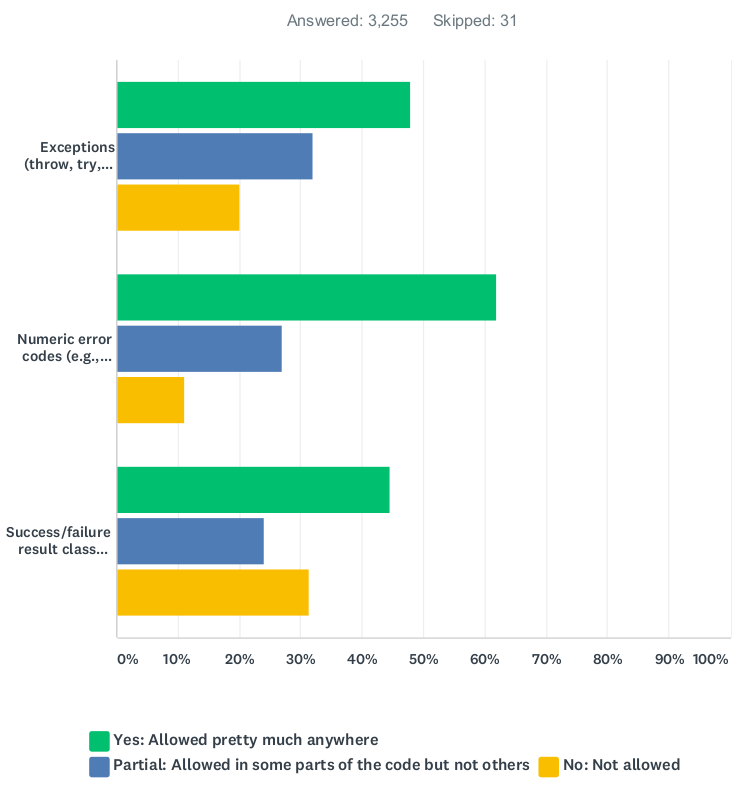
\includegraphics[width=.45\linewidth]{survey_results.png}
	\end{center}
	\end{uncoverenv}
	
\end{frame}

\section{C++ - zero overhead rule}

\begin{frame}{What is zero overhead?}
	\begin{itemize}[<+- | alert@+>]
		\item language features {\color{amethyst}can} introduce overhead
		\item "you don't pay for what you don't use"
		\item if you use a feature it should be as afficient as handcoded version.
	\end{itemize}
\end{frame}

\begin{frame}{Exceptions not to the rescue}
		\centering
		\textcolor{red}{Exceptions break the zero overhead rule.}
		
		But why?
\end{frame}

\section{Exceptions - how do they work?}

\begin{frame}{Approaches towards implementation}
	Two major kinds of implementation:
	\begin{itemize}[<+- | alert@+>]
		\item additional data added to the frame stack
		\item additional data added to someplace on the heap
	\end{itemize}
\end{frame}
	
\begin{frame}{Implementations' consequences}
	\centering
	\begin{tabular}{p{3cm}|p{3cm}|p{3cm}}
		\multirow{2}{*}{implementation}& \multicolumn{2}{c}{performance} \\
		& without throwing & with throwing  \\ \hline \hline
		frame-based  & overhead & fast \\ \hline
		table-based & almost no overhead & slow \\ \hline
	\end{tabular}

	\vskip 1em

	\centering
	\pause
	\begin{alertblock}{Binary size}
		No matter what's the strategy for exception handling. The binary will grow even if you do not use exceptions.
	\end{alertblock}
	
\end{frame}


\begin{frame}{Exceptions summary}
	\begin{columns}[T]
		\begin{column}{0.48\linewidth}
			Pros
			\begin{itemize}[<+- | alert@+>]
				\item differentiated error and success paths
				\item automagical error propagation
				\item little/no boilerplate code
			\end{itemize} \pause
		\end{column}
	\begin{column}{0.48\linewidth}
			Cons
			\begin{itemize}
				\item Performance
				\begin{itemize}[<+- | alert@+>]
					\item slow
					\item not deterministic speed
					\item not deterministic storage occupation
					\item not compatible with C
					\item not usable in any safety standards (e.g. MISRA)
				\end{itemize}
			\end{itemize}
	\end{column}
	\end{columns}
\end{frame}

\section{Possible future of error handling.}

\begin{frame}{Perfect error handling mechanism}
	\centering
	\begin{tabular}{|c|c|c|}
		\hline
		feature & exceptions & std::error\_code \\ \hline \hline
		distinct error path & yes & no \\ \hline
		distinct success path & yes & no \\ \hline \hline
		unhandled error propagation & yes & no \\ \hline
		unhandled error is visible & no & yes \\ \hline
		uncluttered business logic & yes & no \\ \hline \hline
		RTTI required & yes & no \\ \hline
		deterministic space/time occupation & no & yes \\ \hline
		time cost == return & no & yes \\ \hline \hline
		C compatibility & no & no \\ \hline
	\end{tabular}
\end{frame}

\begin{frame}{Key idea for improvement}
	\begin{block}{Key ideas}
		\begin{itemize}[<+- | alert@+>]
			\item Let's use the return channel to return the std::error
			\item Let the compiler generate boilerplate code for error propagation
		\end{itemize}
	\end{block}
	Let's call those \emph{\color{amethyst}static exceptions}
\end{frame}
	
\begin{frame}[fragile]{How to use return channel for std::error}
	\begin{columns}[T]
		\begin{column}{0.48\linewidth}
			We can do that manually using variant:
			\begin{minted}{c++}
using Result = 
      variant<T, std::error>;			
Result foo();
			\end{minted}
		\end{column}
		\begin{column}{0.48\linewidth}
			But this can be nicer with syntax sugar:
			\begin{minted}{c++}
T foo() throws;
			\end{minted}
		\end{column}
	\end{columns}
\end{frame}

\begin{frame}[fragile]{Static exceptions example}
	\begin{onlyenv}<1>
	\begin{minted}[highlightlines={10-11}]{c++}
string f() throws {
  if (flip_a_coin()) throw arithmetic_error::something;
  return "xyzzy"s + "plover"; 
}

string g() throws { return f() + "plugh"; } 

int main() {
  try {
    auto result = g();
    cout << "success, result is: " << result;
  } catch(error err) {
    cout << "failed, error is: " << err.error();
  }
}
	\end{minted}
	\end{onlyenv}

	\begin{onlyenv}<2>
	\begin{minted}[highlightlines={6}]{c++}
string f() throws {
  if (flip_a_coin()) throw arithmetic_error::something;
  return "xyzzy"s + "plover"; 
}

string g() throws { return f() + "plugh"; } 

int main() {
  try {
    auto result = g();
    cout << "success, result is: " << result;
  } catch(error err) {
    cout << "failed, error is: " << err.error();
  }
}
	\end{minted}
	\end{onlyenv}

	\begin{onlyenv}<3>
	
	\begin{minted}[highlightlines={0-4}]{c++}
string f() throws {
  if (flip_a_coin()) throw arithmetic_error::something;
  return "xyzzy"s + "plover"; 
}

string g() throws { return f() + "plugh"; } 

int main() {
  try {
    auto result = g();
    cout << "success, result is: " << result;
  } catch(error err) {
    cout << "failed, error is: " << err.error();
  }
}
	\end{minted}
	\end{onlyenv}

	\begin{onlyenv}<4>
	\begin{minted}[highlightlines={12}]{c++}
string f() throws {
  if (flip_a_coin()) throw arithmetic_error::something;
  return "xyzzy"s + "plover"; 
}

string g() throws { return f() + "plugh"; } 

int main() {
  try {
    auto result = g();
    cout << "success, result is: " << result;
  } catch(error err) {
    cout << "failed, error is: " << err.error();
  }
}
	\end{minted}
	\end{onlyenv}

\end{frame}

\begin{frame}[fragile]{Compiler's support in handling errors}

	\begin{onlyenv}<1>
	\begin{minted}[highlightlines={1-2}]{c++}
int f1() throws;	
int f2() throws;

int main(){
// return f1() + f2(); // error
try return f1() + f2();// ok, covers both 
return try f1()+ f2();
}
	\end{minted}
	\end{onlyenv}

	\begin{onlyenv}<2>
	\begin{minted}[highlightlines={5}]{c++}
int f1() throws;	
int f2() throws;

int main(){
// return f1() + f2(); // error
try return f1() + f2();// ok, covers both 
return try f1()+ f2();
}
	\end{minted}
	\end{onlyenv}

	\begin{onlyenv}<3>
	\begin{minted}[highlightlines={6}]{c++}
int f1() throws;	
int f2() throws;

int main(){
// return f1() + f2(); // error
try return f1() + f2();// ok, covers both 
return try f1()+ f2();
}
	\end{minted}
	\end{onlyenv}

	\begin{onlyenv}<4>
	\begin{minted}[highlightlines={7}]{c++}
int f1() throws;	
int f2() throws;

int main(){
// return f1() + f2(); // error
try return f1() + f2();// ok, covers both 
return try f1()+ f2();
}
	\end{minted}
	\end{onlyenv}

\end{frame}

\begin{frame}{Cool! But what about C compatibility}
	\begin{alertblock}{C compatibility}
 		It is possible, that C will be compatible with static exceptions!
	\end{alertblock}

	
	This implies:
	
	\begin{itemize}
		\item Exceptions could be thrown from C++, passed through C and catched again in C++
		\item We could handle C++ exceptions in C
		\item We could handle C exceptions in C++
	\end{itemize}
\end{frame}

\begin{frame}[fragile]{Short story about C language}
	\begin{minted}{c++}
_Either(int, std_error) somefunc(int a){
  return a > 5 ? _Expected(a) : _Unexpected(a);
}

// ...

_Either(int, std_error) ret = somefunc(a);
if(ret)
  printf("%d\n", ret.expected);
else
  printf("%f\n", ret.unexpected);
	\end{minted}
\end{frame}

\begin{frame}{Static exceptions summary}
\centering
	\begin{tabular}{|c|c|}
		\hline
		feature & static exceptions \\ \hline \hline
		distinct error path & yes \\ \hline
		distinct success path & yes \\ \hline \hline
		unhandled error propagation & yes \\ \hline
		unhandled error is visible & yes \\ \hline
		uncluttered business logic & yes \\ \hline \hline
		RTTI required & no \\ \hline
		deterministic space/time occupation & yes \\ \hline
		time cost == return & yes \\ \hline \hline
		C compatibility & maybe \\ \hline
	\end{tabular}
\end{frame}

\begin{frame}{Possible issue}
	We will end up having 3 ways to handle error codes:
	\begin{itemize}
		\item dynamic exceptions
		\item static exceptions
		\item old style error codes
	\end{itemize}

	\vfill
\end{frame}

\begin{frame}{Bibliography}
	This presentation wouldn't be possible without:
	
	\begin{itemize}
		\item Herb Sutter - author of the proposal (code examples, exception features taken from his proposal) -  \href{http://www.open-std.org/jtc1/sc22/wg21/docs/papers/2018/p0709r1.pdf}{p0709r1}
		
		\item Andrzej Krzemiński for his blog about error codes and error conditions -  \href{https://akrzemi1.wordpress.com/2017/07/12/your-own-error-code/}{Your own error code}
	\end{itemize}
\end{frame}

\begin{frame}{Thank you}
	\begin{center}
		Thank you for your attention!
		\vskip 1em
		Questions?
	\end{center}
	
	\hrule
	\vfill
	
	blog: \href{https://blog.panicsoftware.com}{\alert{blog.panicsoftware.com}} \\
	presentation: \href{https://github.com/dawidpilarski/error_handling_presentation}{\alert{github.com/dawidpilarski/error\_handling\_presentation}}
	
	
	
	
\end{frame}

\end{document}
